\documentclass[a4paper,11pt]{article}

\usepackage[french]{babel}
\usepackage[utf8]{inputenc}
\usepackage[T1]{fontenc}
\usepackage{lmodern}
\usepackage{hyperref}
\usepackage{graphicx}
\usepackage{xcolor}
\usepackage{geometry}

\geometry{margin=2.5cm}

\hypersetup{
    colorlinks=true,
    linkcolor=blue,
    filecolor=magenta,      
    urlcolor=cyan,
    pdftitle={Rapport final - Projet ClimaGraph},
    pdfauthor={Stephene WANTCHEKON et Spero TESSY},
}

\title{
    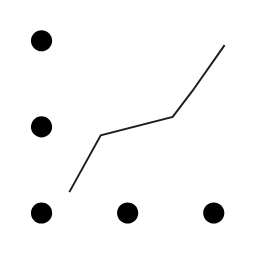
\includegraphics[width=5cm]{../ui/assets/img/logo.png}\\[1cm]
    \textbf{Rapport final - Projet ClimaGraph}\\
    \large{Application de visualisation des données de température et d'humidité}
}
\author{Spero TESSY \\ Stephene WANTCHEKON }
\date{\today}

\begin{document}

\maketitle

\begin{abstract}
Ce document présente les conclusions du projet ClimaGraph, une application développée pour l'analyse et la visualisation des données de température et d'humidité. L'application permet aux utilisateurs d'importer des données depuis différentes sources, de générer des graphiques d'amplitude thermique et hydrique, et d'exporter les résultats pour une utilisation dans des rapports scientifiques. Ce projet a été réalisé par une petite équipe de statisticiens et de programmeurs.
\end{abstract}

\section{Introduction}

Le projet ClimaGraph a été développé pour répondre au besoin d'analyse des données environnementales collectées par des capteurs de température et d'humidité. L'objectif principal était de créer une interface utilisateur intuitive permettant aux chercheurs et aux professionnels de visualiser rapidement les tendances et les écarts au point de rosée, facilitant ainsi l'identification des risques de condensation dans les bâtiments.

\section{Fonctionnalités implémentées}

L'application ClimaGraph offre les fonctionnalités suivantes:

\begin{itemize}
    \item Importation de données depuis différents formats (Excel, CSV)
    \item Visualisation des écarts au point de rosée quotidiens
    \item Analyse des amplitudes thermiques et hydriques avec représentation graphique
    \item Identification des zones à risque de condensation (écart < 3°C)
    \item Profils d'humidité par capteur
    \item Températures moyennes quotidiennes par capteur
    \item Exportation des graphiques en formats PNG
    \item Interface utilisateur multiplateforme (Windows et macOS)
\end{itemize}

\section{Architecture technique}

L'application a été développée en Python avec les bibliothèques suivantes:
\begin{itemize}
    \item pywebview pour l'interface utilisateur
    \item Matplotlib pour la génération des graphiques
    \item Pandas pour la manipulation des données
    \item NumPy pour les calculs scientifiques
    \item etc... 
\end{itemize}

L'architecture modulaire du projet permet une maintenance facile et l'ajout de nouvelles fonctionnalités. Notre équipe de statisticiens et de programmeurs a travaillé en étroite collaboration pour assurer la précision des calculs et l'ergonomie de l'interface.

\section{Résultats et exemples}

Les graphiques générés par ClimaGraph permettent d'identifier rapidement:
\begin{itemize}
    \item Les périodes où l'écart au point de rosée est inférieur à 3°C (zone rouge)
    \item Les variations saisonnières de l'amplitude hydrique
    \item Les tendances à long terme des conditions environnementales
\end{itemize}

\begin{figure}[h]
    \centering
    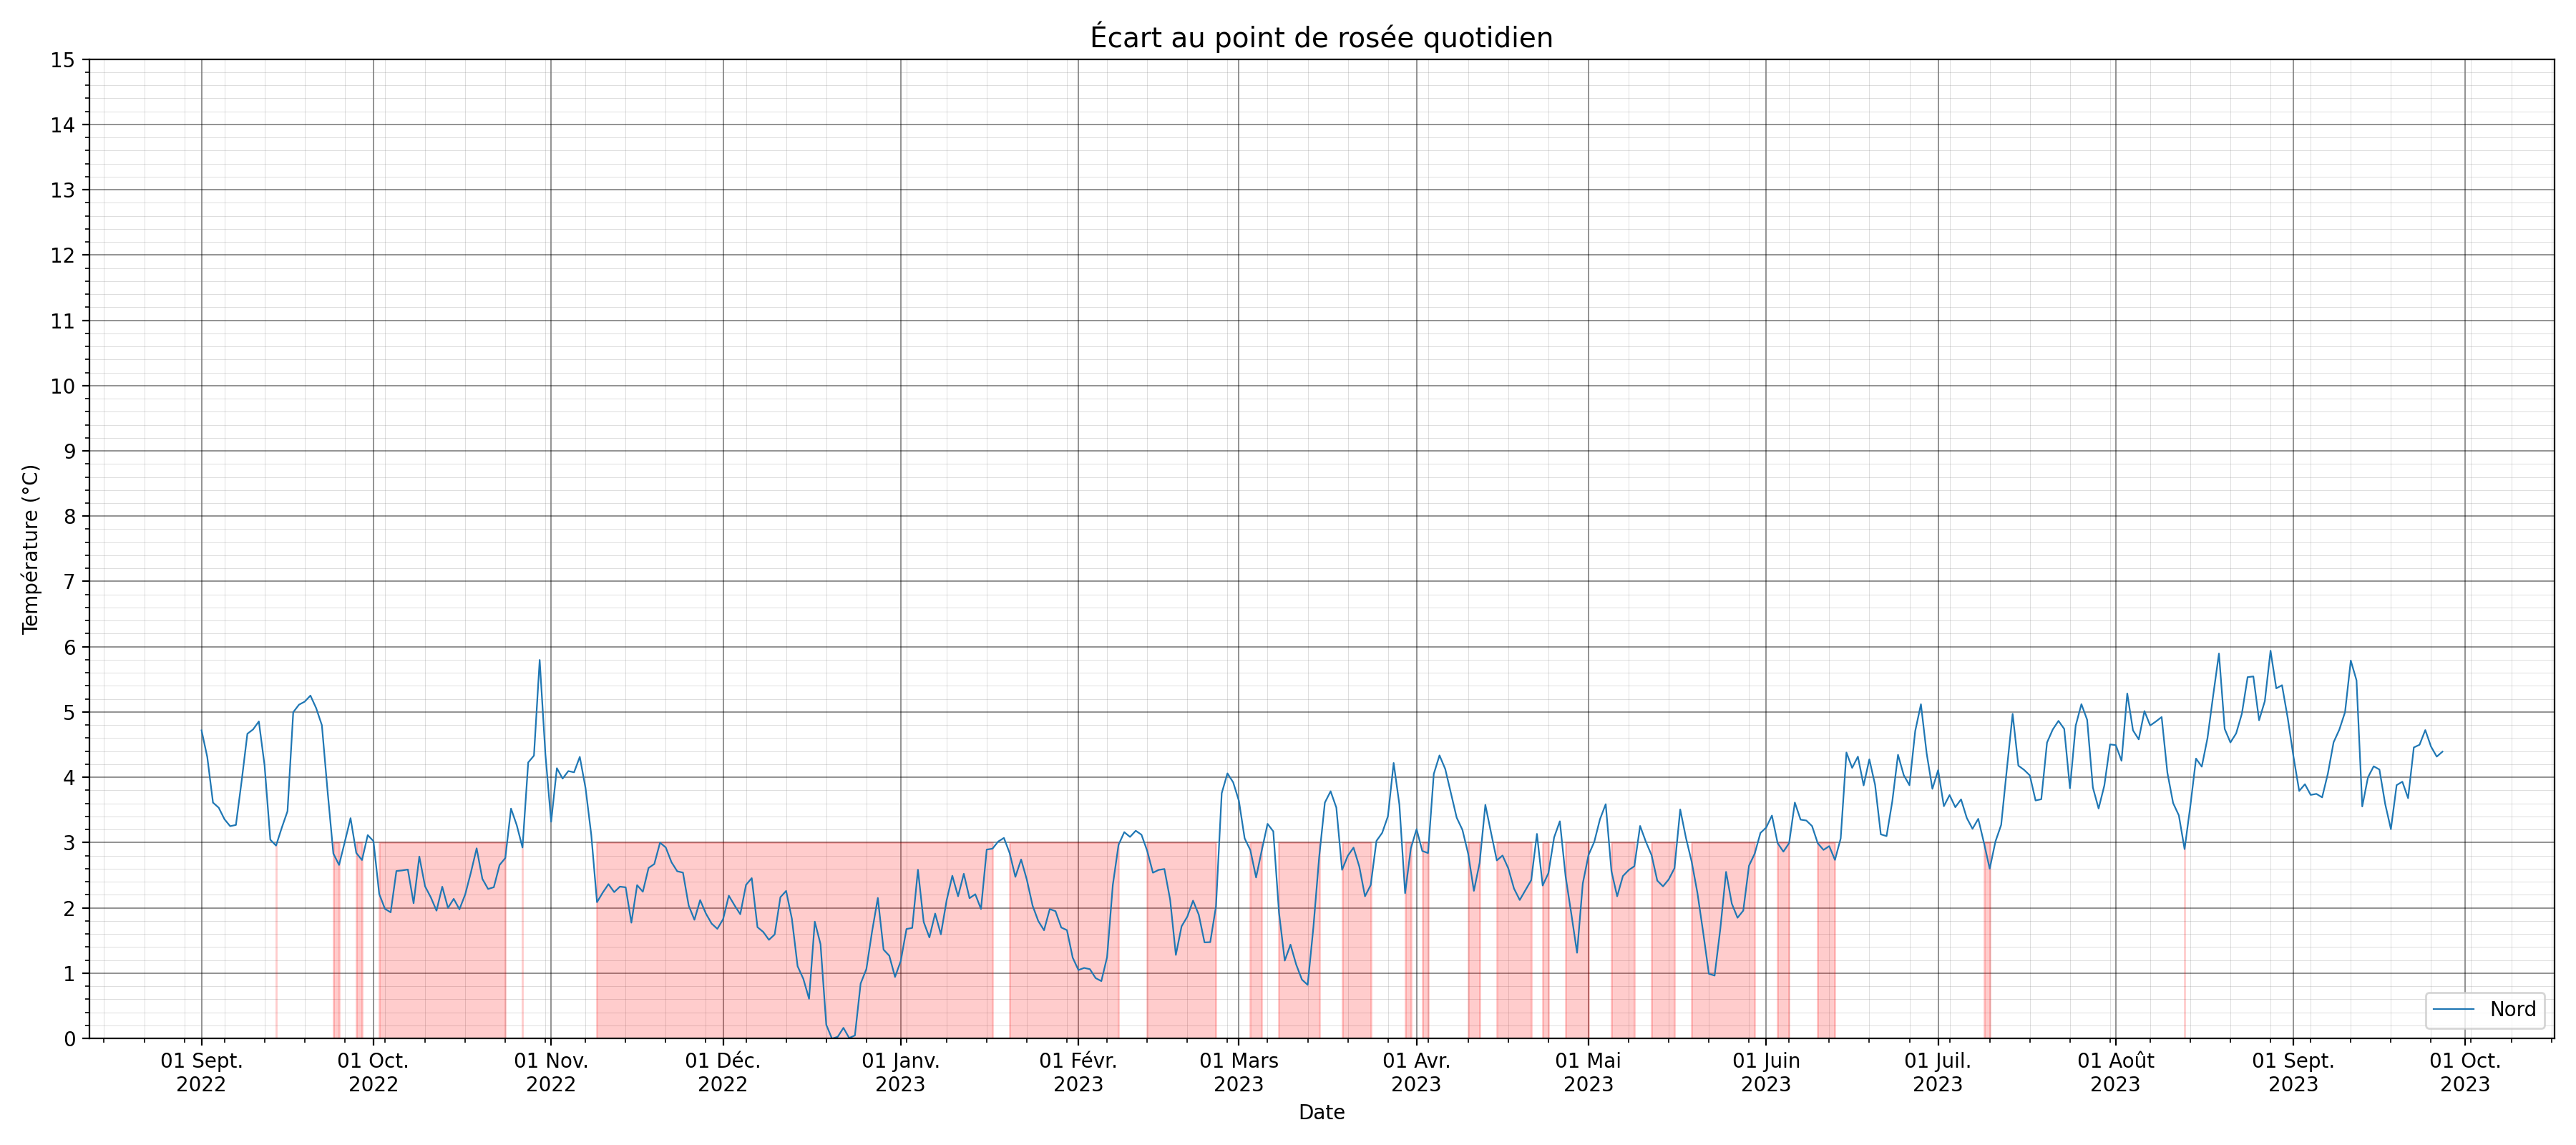
\includegraphics[width=0.8\textwidth]{../screenshots/Écart_au_point_de_rosée_(risque_de_condensation)-id-dew_point_risk-20250506_143243.png}
    \caption{Écart au point de rosée avec identification des zones à risque de condensation}
\end{figure}

\begin{figure}[h]
    \centering
    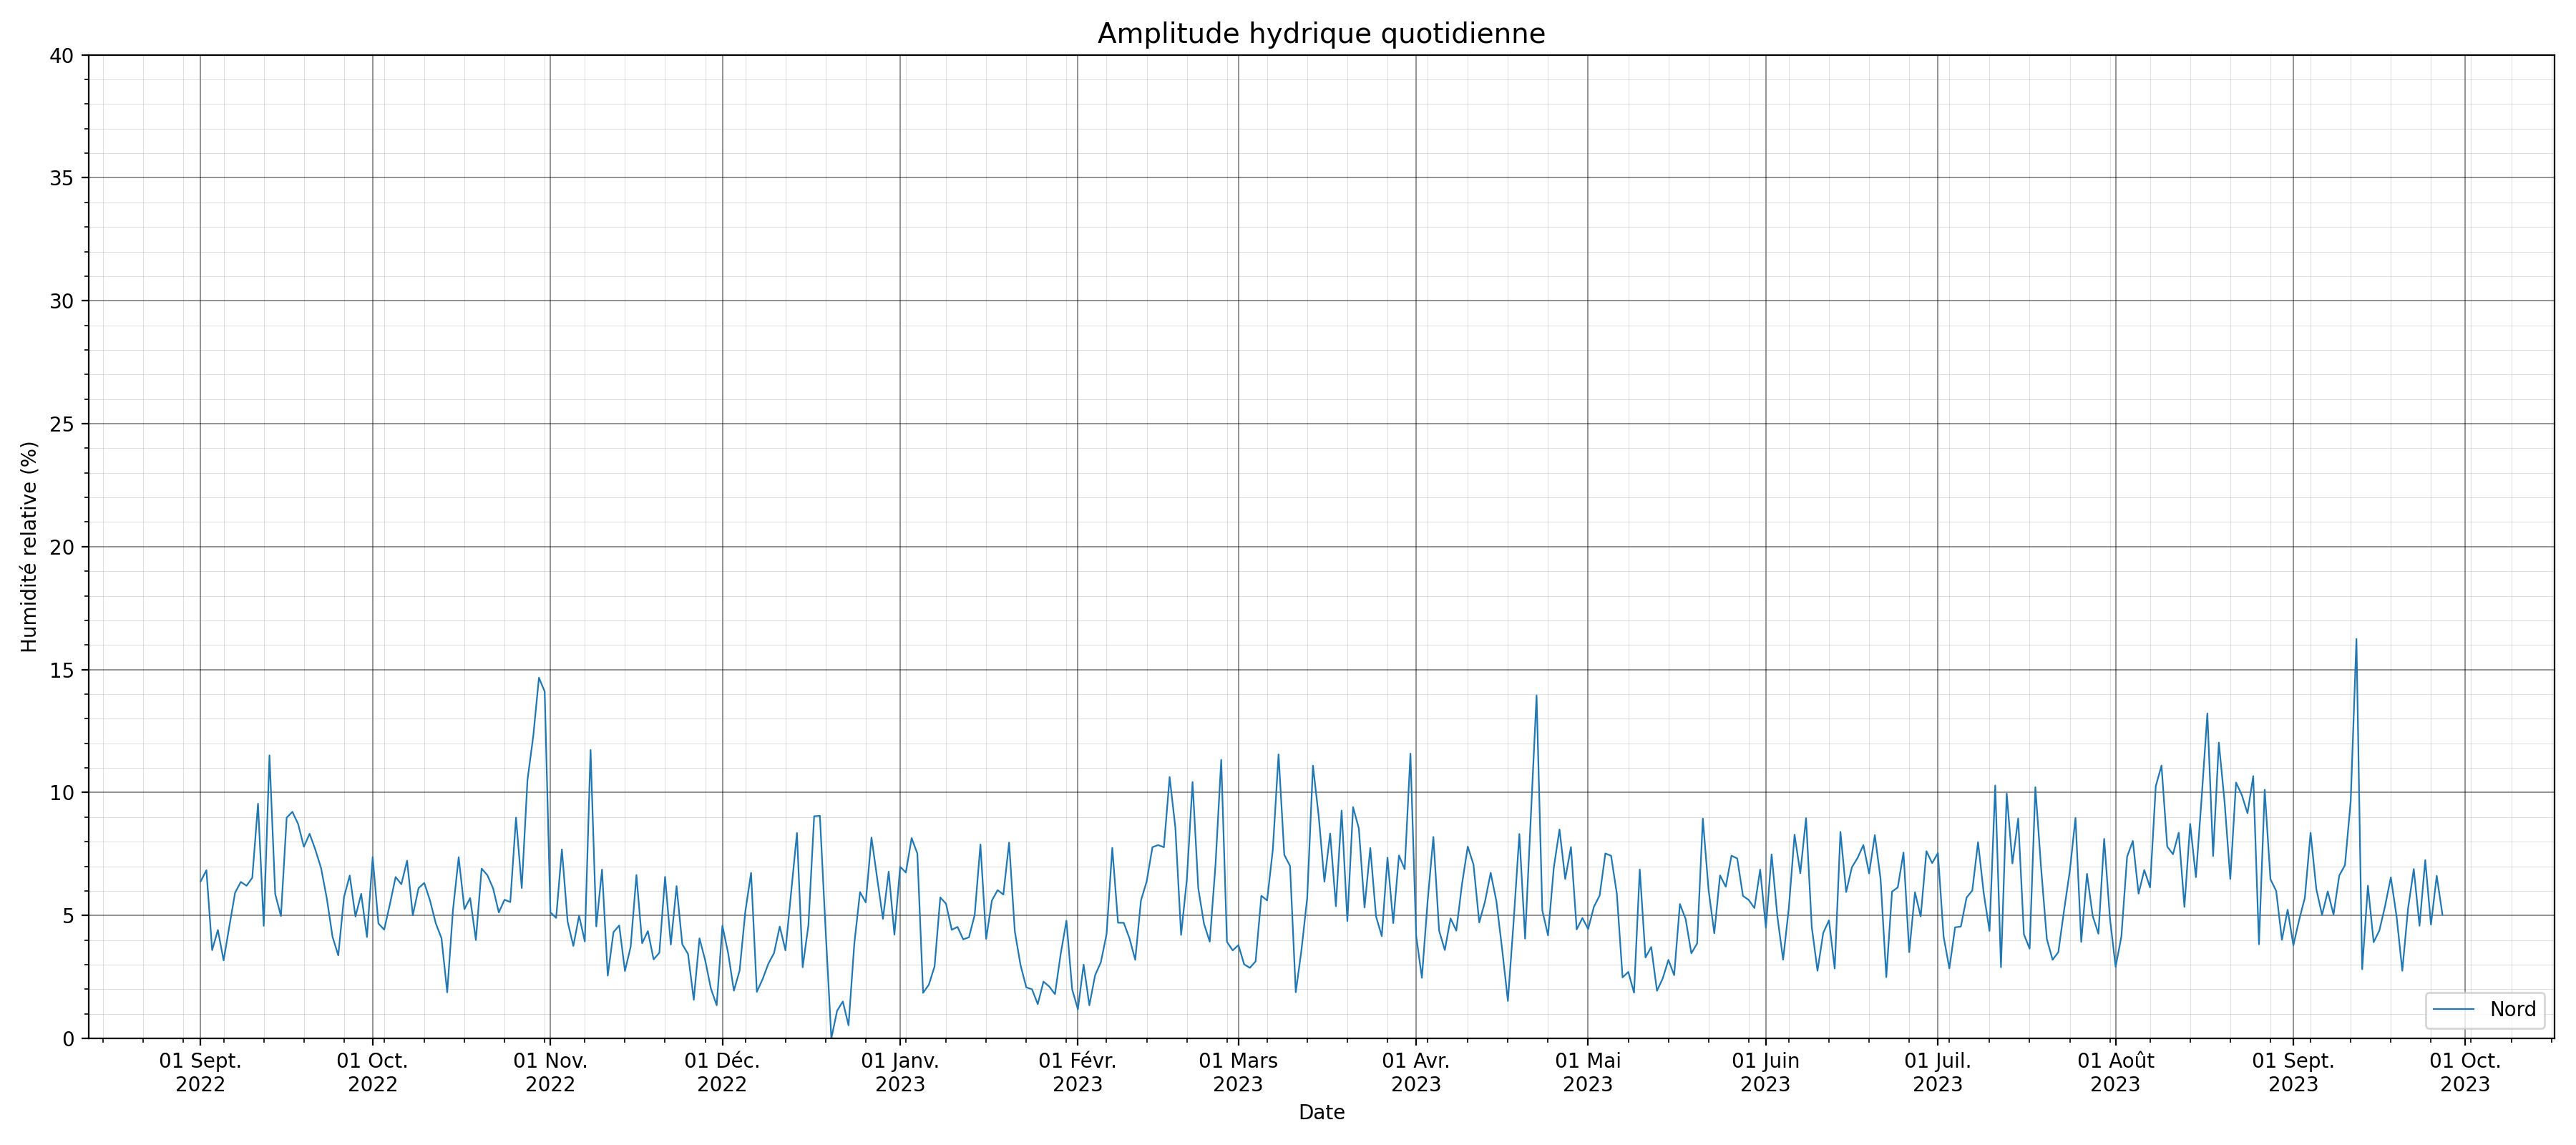
\includegraphics[width=0.8\textwidth]{../screenshots/Amplitude_hydrique_quotidienne-id-humidity_amplitude-20250506_143243.png}
    \caption{Analyse de l'amplitude hydrique quotidienne}
\end{figure}

\newpage

\begin{figure}[h]
    \centering
    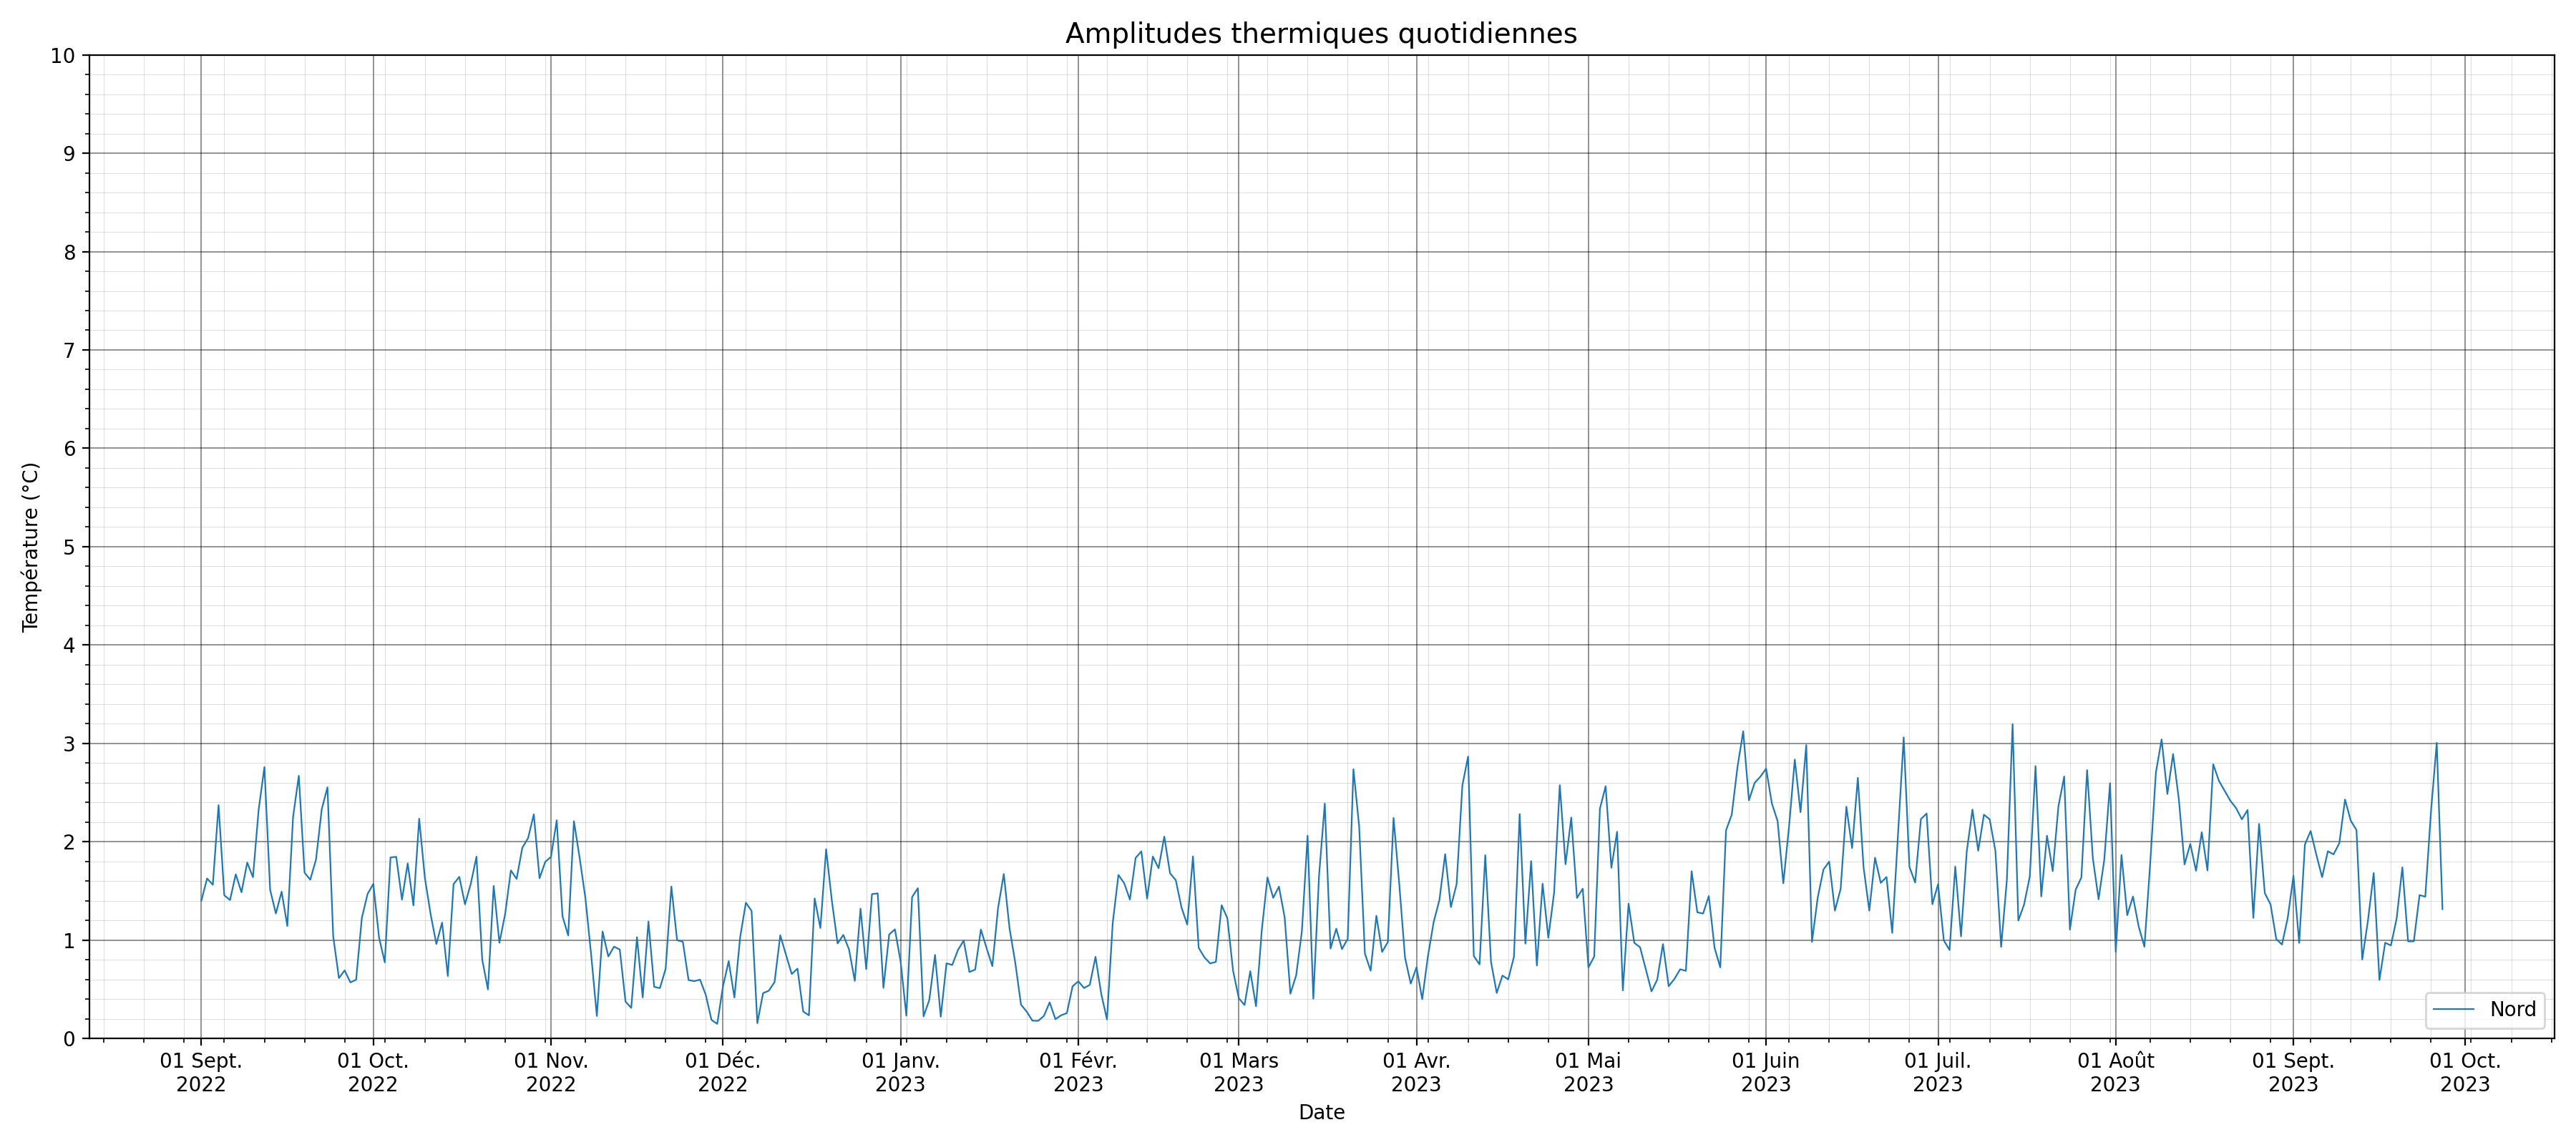
\includegraphics[width=0.8\textwidth]{../screenshots/Amplitude_thermique_quotidienne-id-temperature_amplitude-20250506_143243.png}
    \caption{Analyse de l'amplitude thermique quotidienne}
\end{figure}

\begin{figure}[h]
    \centering
    \includegraphics[width=0.8\textwidth]{../screenshots/Humidité_en_fonction_du_temps-id-humidity_time-20250506_143243.png}
    \caption{Humidité en fonction du temps}
\end{figure}

\newpage

\begin{figure}[h]
    \centering
    \includegraphics[width=0.8\textwidth]{../screenshots/Profil_d'humidité_par_capteur-id-humidity_profile_per_sensor-20250506_143243.png}
    \caption{Profil d'humidité par capteur}
\end{figure}

\begin{figure}[h]
    \centering
    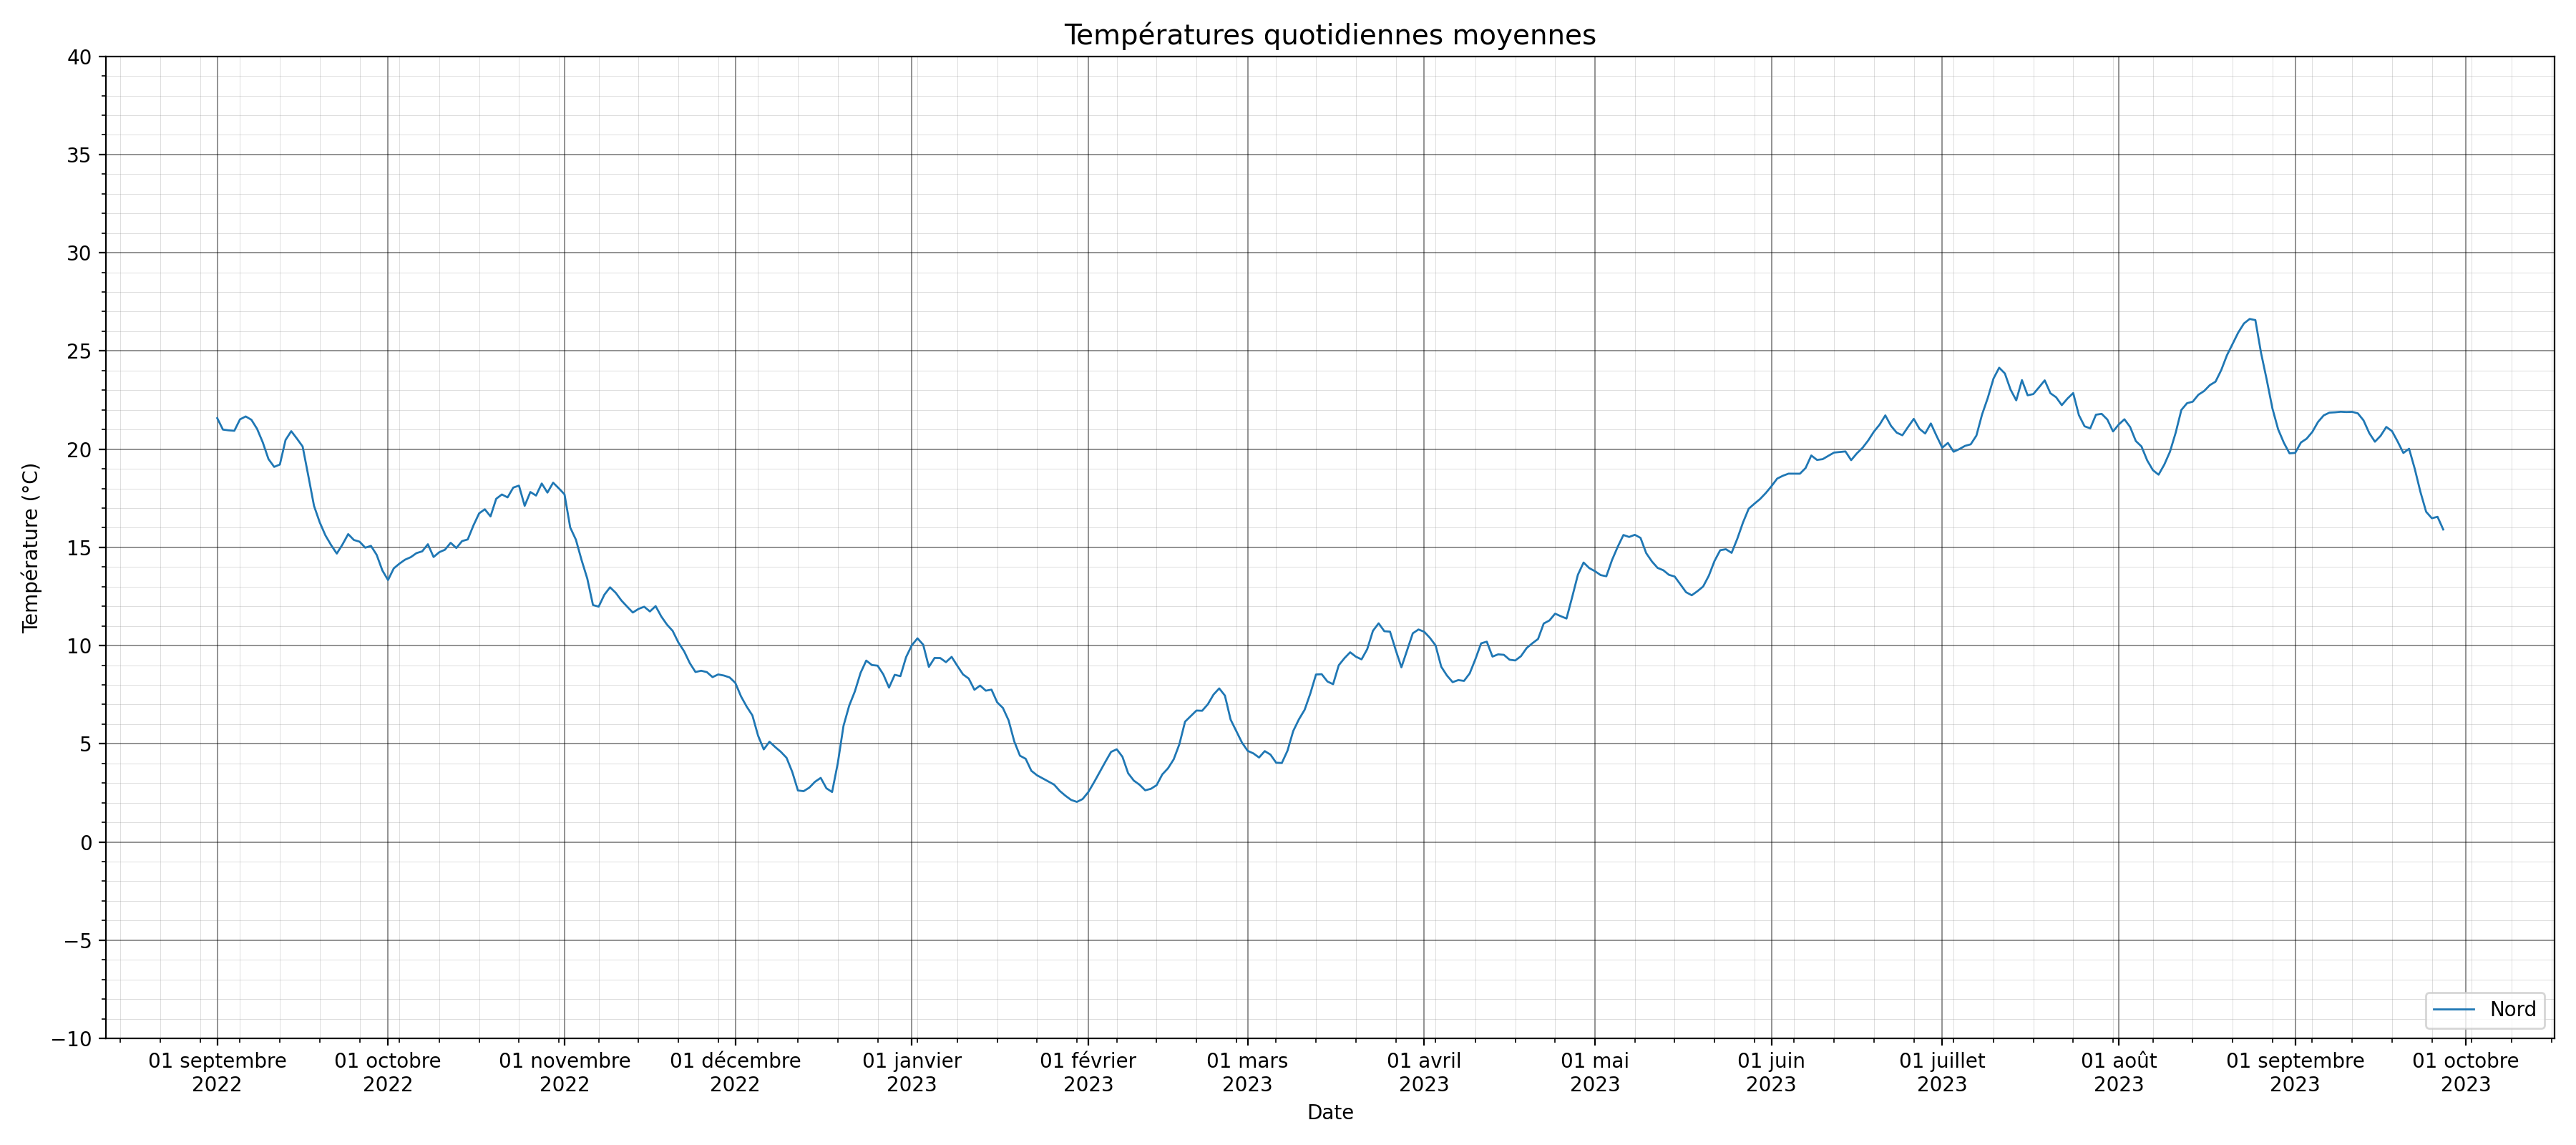
\includegraphics[width=0.8\textwidth]{../screenshots/Températures_quotidiennes_(Température_en_fonction_du_temps)-id-temperature_time-20250506_143243.png}
    \caption{Températures quotidiennes en fonction du temps}
\end{figure}

\newpage

\begin{figure}[h]
    \centering
    \includegraphics[width=0.8\textwidth]{../screenshots/Température_moyenne_quotidienne_par_capteur_1-Capteur---20250424_165815.png}
    \caption{Température moyenne quotidienne par capteur}
\end{figure}

\begin{figure}[h]
    \centering
    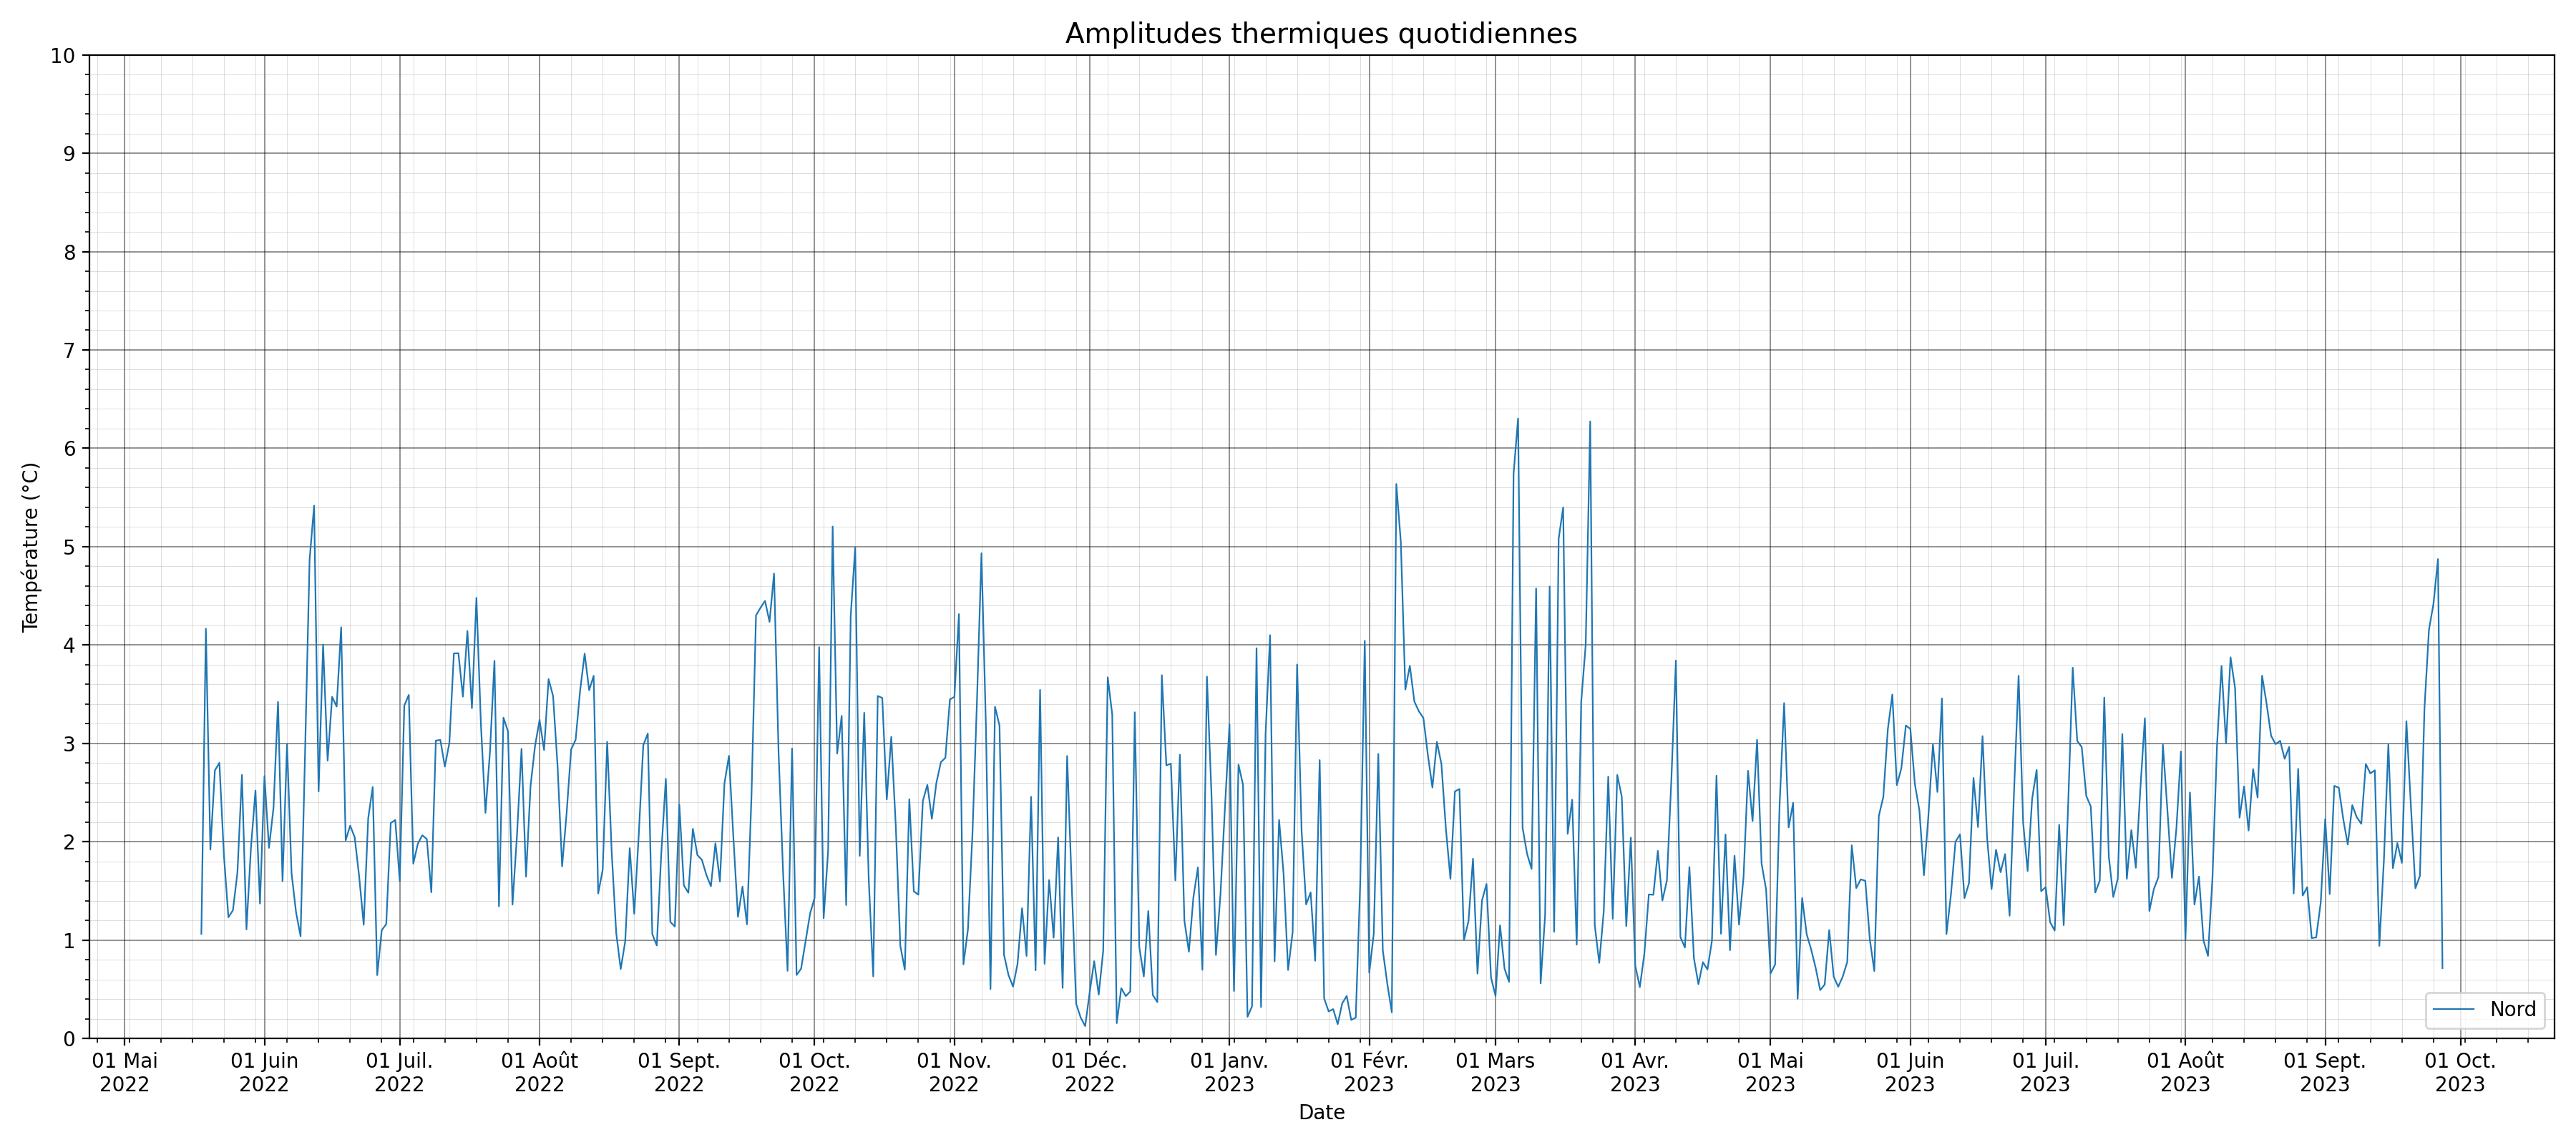
\includegraphics[width=0.8\textwidth]{../screenshots/Amplitude_thermique_quotidienne_1-Capteur---20250427_112247.png}
    \caption{Amplitude thermique quotidienne par capteur}
\end{figure}


\newpage
\section{Téléchargement de l'application}

L'application ClimaGraph est maintenant disponible pour macOS. Pour télécharger l'application, cliquez sur le lien suivant:

\begin{center}
\colorbox{gray!20}{
\begin{minipage}{0.8\textwidth}
\vspace{0.3cm}
\centering
\Large{\href{https://github.com/stephene369/TemperatureGraphMacProgramm/raw/main/ClimaGraph.zip}{Télécharger ClimaGraph pour macOS}}
\vspace{0.3cm}
\end{minipage}
}
\end{center}

\subsection{Instructions d'installation}
\begin{enumerate}
    \item Téléchargez le fichier \texttt{ClimaGraph.zip} en cliquant sur le lien ci-dessus
    \item Double-cliquez sur le fichier téléchargé pour le décompresser
    \item Double-cliquez sur l'application \texttt{ClimaGraph.app} pour la lancer
\end{enumerate}

\textbf{Note:} Lors du premier lancement, macOS pourrait afficher un message de sécurité. Dans ce cas, faites un clic droit (ou Ctrl+clic) sur l'application, sélectionnez "Ouvrir" dans le menu, puis confirmez que vous souhaitez ouvrir l'application.

\section{Conclusion et perspectives}

Le projet ClimaGraph a atteint ses objectifs en fournissant une solution complète pour l'analyse des données de température et d'humidité. Les utilisateurs peuvent désormais visualiser rapidement les tendances et identifier les zones à risque de condensation.

Pour les développements futurs, nous envisageons:
\begin{itemize}
    \item L'ajout de fonctionnalités d'analyse statistique avancée
    \item L'intégration avec des services cloud pour le stockage des données
    \item L'implémentation d'un système d'alerte en temps réel
    \item L'intégration de modèles prédictifs basés sur l'apprentissage automatique
\end{itemize}




\section*{Remerciements}

Nous tenons à exprimer notre sincère gratitude à notre client pour sa confiance, sa patience et sa collaboration tout au long de ce projet.  

Votre implication et vos retours réguliers ont été essentiels pour faire évoluer l’application et aboutir à une solution répondant à vos besoins. Nous espérons que ClimaGraph vous apportera entière satisfaction dans vos analyses.




\end{document}
